% Generated by Sphinx.
\documentclass[a4paper,10pt,english]{manual}
\usepackage[utf8]{inputenc}
\usepackage[T1]{fontenc}
\usepackage{babel}
\usepackage{times}
\usepackage[Bjarne]{fncychap}
\usepackage{sphinx}
\usepackage{picins}

\usepackage{hyperref}
\usepackage{fontspec}
\usepackage{xunicode}
\usepackage{xltxtra}
\XeTeXlinebreaklocale "zh"
\XeTeXlinebreakskip = 0pt plus 1pt
\setsansfont{Vera Sans YuanTi Mono}
\setromanfont{Vera Sans YuanTi Mono}

%标题控制
\titleformat{\chapter}[hang]{\huge\filcenter}{}{1em}{}[\thispagestyle{empty}]
\titlespacing{\chapter}{0pt}{-21pt}{18pt}

%\setlength{\textheight}{9.5in}
%\newsectionwidth{0pt} 

\begin{document}
%\begin{resume}


\chapter{个人简历}


\section{基本资料}
%\begin{figure}[!h]
%\begin{flushright}
%  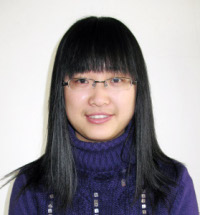
\includegraphics[height=5cm]{mypic.jpg}
%\end{flushright}
%\end{figure}
  	
\parpic[r]{
  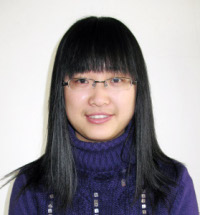
\includegraphics[height=5cm]{mypic.jpg}}

\begin{itemize}
\item {} 
姓名: 盛艳

\item {} 
性别: 女

\item {} 
出生年月: 1985年8月

\item {} 
籍贯: 苏州

\item {} 
健康状况: 优秀

\item {} 
毕业院校: \href{http://www.yzu.edu.cn}{扬州大学} 信息工程学院

\item {} 
专业/方向: 计算机应用技术/数据挖掘

\item {} 
学历: 硕士/2010年七月毕业

\item {} 
手机: 13813147410

\item {} 
Email: \href{mailto:shengyan1985@gmail.com}{shengyan1985@gmail.com}

\item {} 
通信地址: 江苏省扬州大学信息工程学院400173\#

\end{itemize}

\section{工作意向}
\begin{itemize}
\item {} 
软件开发工程师;

\item {} 
Web开发工程师;


\end{itemize}


\section{英语水平}
\begin{itemize}
\item {} 
于2004年获得CET-4证书;

\item {} 
具有扎实的英语应用能力及较强的计算机专业英文文献阅读及翻译水平, 并已发表多篇英文学术论文.

\end{itemize}


\section{计算机能力/技能}
\begin{itemize}
\item {} 
精通 \href{http://www.python.org/}{Python}, 熟练使用基本Python库; C/C++相关基础知识扎实;

\item {} 
熟悉Web应用开发; 熟练掌握Html, CSS, Javascript等Web技术, 并熟练使用 \href{http://jquery.com}{JQuery}, 有Ajax开发经验;

\item {} 
掌握 \href{http://www.djangoproject.com/}{Django} 框架, 熟悉 \href{http://karrigell.sourceforge.net/}{Karrigell};

\item {} 
熟悉 \href{http://www.mysql.com}{MySQL}, \href{http://www.sqlite.org}{Sqlite} 等数据库使用;

\item {} 
熟悉Linux/Unix类操作系统系统管理及维护;

\item {} 
具有较扎实的算法理论知识;

\item {} 
具有较强的理解问题, 分析问题能力, 对未知问题具有潜在的好奇心并不断通过各种方式找到解决方案;

\item {} 
具有良好的编程风格, 对编码规范及文学化编程比较熟悉.

\end{itemize}


\section{教育经历}
\begin{itemize}
\item {} 
2007年9月\textasciitilde{}至今: 以优异成绩推荐免试于扬州大学信息工程学院, 攻读计算机应用技术专业/数据挖掘方向硕士学位, 现已完成前期基础课程的学习;

\item {} 
2003年9月\textasciitilde{}2007年7月: 于扬州大学信息工程学院, 攻读计算机科学与技术(师范)专业学士学位, 完成本科阶段学习.

\end{itemize}


\section{主修课程}
\begin{itemize}
\item {} \begin{description}
\item[本科阶段(2003年8月\textasciitilde{}2007年6月)]
\emph{基础课程:} 高等数学, 离散数学, 概率论与数理统计, 线性代数, PASCAL语言程序设计, C语言程序设计, C++程序设计, 汇编语言, 数据结构, 操作系统原理, 计算方法, 计算机通信, 编译原理, 数据库原理及应用, 面向对象技术, 计算机网络, 软件工程, 多媒体技术, 人工智能, 数字图像处理, 计算机组成原理, 微机原理, 单片机原理;

\end{description}

\item {} \begin{description}
\item[研究生阶段(2007年8月\textasciitilde{}2008年7月)]
\emph{基础课程:} 矩阵论, 数据仓库, 数据挖掘, 分布式数据库原理, 并行处理技术, 并行算法设计与分析, 计算机体系结构, 计算机网络技术, 最优化理论;

\emph{研究方向:} 数据挖掘, 概念格, 文本信息检索等. 熟悉多种数据挖掘算法及理论, 如: 经典Apriori, Decision Tree分类, 朴素贝叶斯分类, KNN分类, KMeans聚类, Rough Set Theory, Fuzzy Set Theory及形式概念分析中的Godin, Bordat算法等.

\end{description}

\end{itemize}


\section{发表论文}
\begin{itemize}
\item {} 
SHENG Yan, LI Yun, TIAN Su-fang, LUAN Luan. A Rough Concept Lattice Model of Variable Precision. IEEE International Symposium on Intelligent Information Technology Application 2008 (IITA'08), Shanghai City, China;

\item {} 
Yun Li, Yan Sheng, Luan Luan, Lianglei Sun and Ling Chen. A Personalized Search Results Ranking Method Based on WordNet. 8th IEEE/ACIS International Conference on Computer and Information Science (ICIS 2009), June 1-3, 2009, Shanghai, China;

\item {} 
Li Yun, Sheng Yan, Luan Luan. A Text Classification Method with an Effective Feature Extraction based on Category Analysis.

\item {} 
盛艳, 李云, 李拓, 袁运浩. 一种基于概念格模型的本体合并方法. 2008全国开放式分布与并行计算学术年会(DPCS2008), 2008年10月25\textasciitilde{}27日;

\item {} 
盛艳, 李云, 李拓, 栾鸾. 基于概念格模型的本体映射. 第三届江苏计算机大会(Jiangsu Computer Conference 2008, JSCC 2008), 2008年11月14日\textasciitilde{}16日; 此论文被评为第三届江苏计算机大会"优秀论文";

\item {} 
栾鸾, 李云, 盛艳. 多关系频繁项集的并行获取. 2008全国开放式分布与并行计算学术年会(DPCS2008), 2008年10月25\textasciitilde{}27日;

\end{itemize}

上述论文可在 \href{http://github.com/lizzie/lizworkspace/tree/cb82ad8d84a1b1a12df80e3508e3629abf09ac83/paper}{这里} 找到.


\section{奖励/证书}
\begin{itemize}
\item {} 
2003\textasciitilde{}2004学年获一等专业奖学金;

\item {} 
2003\textasciitilde{}2004学年被评为院"三好学生";

\item {} 
2004\textasciitilde{}2005学年获二等专业奖学金;

\item {} 
2004\textasciitilde{}2005学年被评为校"三好学生";

\item {} 
2005\textasciitilde{}2006学年获朱敬文奖学金;

\item {} 
2005\textasciitilde{}2006学年获校"优秀团员"称号;

\item {} 
2007学年获"优秀毕业生"称号;

\item {} 
2007\textasciitilde{}2008学年获研究生朱敬文奖学金.

\end{itemize}


\section{项目经历}
\begin{itemize}
\item {} 
2007.12\textasciitilde{}2008.3 PR自动化工具
\begin{quote}

\emph{描述:} 由于学校的资料搜索系统涉及到很多脚本和程序文件数量很大, 为了使系统架构更加清晰, 也使开发维护人员更快更容易的理解整个流程, 设计并开发一个自动化脚本分析工具, 最大可能的呈现脚本, 程序, 配置文件之间的调用关系, 以便更好地理解整个系统.

\emph{职责:} Linux下Python实现后台脚本并使用命令行带参数解析模式, 解析输入文件, 将产生的文件之间的调用关系录入Mysql数据库; 前端使用Django开发, 实现查询文件并输出相关的信息(包括该文件调用的c, perl, python, shell脚本, conf配置文件等的图像或文本信息).
\end{quote}

\item {} 
2007.9\textasciitilde{}2008.3 Galicia平台扩展
\begin{quote}

\emph{描述:} Galicia是个开源项目, 在此基础上实现形式概念分析中的一些概念格构造算法, 如Godin算法, Godin改进算法等, 分析算法的时间空间复杂度.

\emph{职责:} 在理解形式概念分析的基础上, 根据概念格自身特性, 掌握基本够格算法并实现, 之后图形显示结果格图, 以便更直观地得到概念格中概念及概念之间的继承关系.
\end{quote}

\item {} 
2008.4\textasciitilde{}2008.11 Openbookproject开放图书计划
\begin{quote}

\emph{描述:} 中文Pythonic技术图书的翻译编写项目, 其工程网址在 \href{http://code.google.com/p/openbookproject/}{http://code.google.com/p/openbookproject}. 其中的LovelyPython是原创图书, 将Python以最易懂的方式介绍给读者, 可作为Python初学者急速入门图书.


\emph{职责:} 参与LovelyPython图书整个创作过程, 具体有: PCS环境篇/语法篇/模块篇中大多数章节的编写, 实例故事练习题设计及解答及各种校对等. 由于此项目是基于google code, 所以非常熟悉分布式团队合作的整个过程.
\end{quote}

\item {} 
2008.11\textasciitilde{}2009.01 禽流感病毒基因组生物信息学分析平台构建
\begin{quote}

\emph{描述:} 针对国际上各大生物信息中心提供的多个分析软件和基因/核酸数据库, 如BLAST检索系统(The Basic Local Alignment Search Tool, 一个基本的局部序列相似性比对搜索工具)及NCBI数据库(National Center for Biotechnology Information, 生物信息数据库中心), SMS2(The Sequence Manipulation Suite 2, 是用于分析较短的DNA和蛋白质序列的教学实验分析工具), Clustalx-2.0.10(用于进行DNA或蛋白质的多序列比对程序)等, 进行本地化生物信息学分析平台的构建, 并在此基础上进行功能扩展, 具体为禽流感病毒基因组数据库的选取, 定时更新及维护, 方便科研人员对禽流感病毒基因进行分析.


\emph{职责:} 完整搭建生物信息分析平台及其扩展. 主要有: 服务器基础环境安装及部署, 采用RedHat Enterprise Linux 4.0 AS作为服务器操作系统, 采用Apache2.2作为Web服务器及相关支持工具的安装. BLAST分析工具的本地化部署及相关数据库的安装, SMS2和Clustalx的安装部署, 并将三者整合起来. 其中, 基于Django0.96进行信息平台扩展并使用mod\_python部署到Apache上形成一整套完整的分析系统. 对系统扩展的工作主要有: 在所有基因数据库中提取禽流感病毒基因并构建二级数据库, 随着NCBI数据库的更新也随之更新并提供扩展检索功能.
\end{quote}

\item {} 
2008.04\textasciitilde{}2009.01 各种使用Python编写的工具程序集
\begin{quote}

\emph{描述:} 包含很多实用和非实用工具程序, 其项目网址为 \href{http://code.google.com/p/lizworkspace/}{http://code.google.com/p/lizworkspace/} . 主要有: Backup(备份两台机子上的监视文件以保持同步), streamdata(流数据上进行频繁项集的挖掘), perm(排列组合算法), mp3\_classify(将mp3歌曲根据歌手分类), powerset(产生集合的幂集), spider(本体实验中写的yahoo爬虫), search(分析google搜索结果用于个性化搜索实验), crontabanalysis(分析crontab文件), rmfilebaseondate(根据文件名上的日期删除文件), XMPP\_Jabber(基于XMPP/Jabber协议的机器人程序), godin(Godin算法, 序列, 模糊集, 粗糙集上的构格算法), FSproj(特征选择相关, 用于文本自动分类), Multi\_Relation(多关系上的贝叶斯分类).
\end{quote}

\end{itemize}


\section{爱好/特长}
\begin{itemize}
\item {} 
看电影, 听英文歌曲, 打羽毛球;

\item {} 
喜欢玩各种图像处理软件和服务, 如PhotoShop, Illustrator, GIMP, Picasa等.

\end{itemize}


\section{自我评价}
\begin{itemize}
\item {} 
责任心比较强, 能吃苦耐劳;

\item {} 
对人比较真诚, 有积极向上的乐观性格, 遇到困难不会轻易妥协;

\item {} 
容易和别人相处, 有比较强的团队精神;

\end{itemize}


\chapter{Liz's Resume}


\section{Basic Info}
%\begin{figure}[!h]
%\begin{flushright}
%  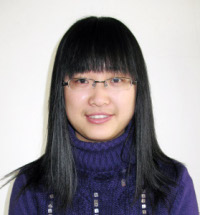
\includegraphics[height=5cm]{mypic.jpg}
%\end{flushright}
%\end{figure}
  	
\parpic[r]{
  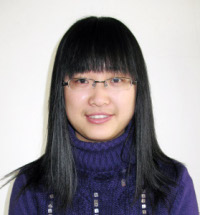
\includegraphics[height=3cm]{mypic.jpg}}

\begin{itemize}

\item {} 
Name: Yan Sheng

\item {} 
Sex: Female

\item {} 
Birthday: 1985, August

\item {} 
Origin: SuZhou

\item {} 
Health status: Excellent

\item {} 
Graduate institutions: Institute of Information Engineering, \href{http://www.yzu.edu.cn}{Yangzhou University}

\item {} 
Professional/Direction: Computer Application Technology/Data Mining

\item {} 
Qualifications: Master/graduated in July 2010

\item {} 
Mobile Phone: 13813147410

\item {} 
Email: \href{mailto:shengyan1985@gmail.com}{shengyan1985@gmail.com}

\item {} 
Communication Address: 400173\#, Institute of Information Engineering, Yangzhou University, JiangSu Province

\end{itemize}

\section{Job Objective}
\begin{itemize}

\item {} 
Software Development Engineer;

\item {} 
Web Development Engineer;

\end{itemize}


\section{English Ability}
\begin{itemize}

\item {} 
In 2004, obtained CET-4 certificate;

\item {} 
Have the good ability of English reading, writing, listening and speaking. Do well in reading or translating English literature of computer science and have published scholarly English papers.

\end{itemize}


\section{Computer Ability and Skill}
\begin{itemize}

\item {} 
Proficient in \href{http://www.python.org/}{Python}, Familiar with the standard Python basis library;

\item {} 
Familiar with the Web application development; Master Html, CSS, Javascript and other Web technologies, and  use \href{http://jquery.com}{JQuery} skilled, also have Ajax development experience;

\item {} 
Become adroit at the \href{http://www.djangoproject.com/}{Django} Web development framework and know about \href{http://karrigell.sourceforge.net/}{Karrigell};

\item {} 
Familiar with the use of \href{http://www.mysql.com}{MySQL}, \href{http://www.sqlite.org}{Sqlite} and other databases;

\item {} 
Familiar with system management and maintenance of Linux/Unix-like operating system;

\item {} 
Know many algorithms widely;

\item {} 
Have better ability to understand and analyze problems and be very curious about the programming-related issues;

\item {} 
Have a good coding style and familiar with the coding rule and Literate Programming.

\end{itemize}


\section{Education}
\begin{itemize}
\item {} 
From September 2007 to now: studying in Institute of Information Engineering, Yangzhou University and doing some research about data mining;

\item {} 
From September 2003 to July 2007: also learned lots of things in Institute of Information Engineering, Yangzhou University and obtained the bachelor's degree of Computer Science and Technology (Normal).

\end{itemize}


\section{Project Experience}
\begin{itemize}
\item {} 
2007.12\textasciitilde{}2008.3 PR
\begin{quote}
\emph{Describe:} In order to understand the call relationships among files(scripts, program source files and configuration files) in the whole system quickly, we designed and developed a script analysis tools automatically. This tool also can search the keyword and print the search results in text or pictures.

\emph{Duties:} The tools has two parts, one is to obtain the relations among lots of files and then save the relations to Mysql database in the backend; The other is a web interface developed by Django to retrieval the files which have certain keyword and related files(including c, perl, python, bash scripts, configuration files and text files).
\end{quote}

\item {} 
2007.9\textasciitilde{}2008.3 Galicia
\begin{quote}

\emph{Describe:} Galicia is an open source project to implement concept lattice construction algorithms.

\emph{Duties:} Improve the Godin algorithms to obtain better time and space complexity.
\end{quote}

\item {} 
2008.4\textasciitilde{}2008.11 Openbookproject
\begin{quote}

\emph{Describe:} The project is about the translation or creatation of Chinese Pythonic books which is hold on \href{http://code.google.com/p/openbookproject/}{http://code.google.com/p/openbookproject}. LovelyPython is a original book which aimed to introduce the python to reader in the most understandable way and it can be a quick entry book for python beginners.

\emph{Duties:} Took part in the whole creative process of LovelyPython. The detail: finished the most of chapters in the first three parts of PCS,  designed the exercises, many proofing works and so on. Since the project is based on the google code, I am very familiar with the whole process of distributed teamwork.
\end{quote}

\item {} 
2008.11\textasciitilde{}2009.01 Construction of Avian virus genome bioinformatics analysis platform
\begin{quote}

\emph{Describe:} Since major international Bioinformatics Center provide many anaysis software for gene and gene/nucleic acid database, such as, BLAST retrieval system(The Basic Local Alignment Search Tool) and NCBI database(National Center for Biotechnology Information), SMS2(The Sequence Manipulation Suite 2, for analyzing the shorter DNA or Protein sequence), Clustalx-2.0.10(Used for DNA or multiple protein sequence alignment tool), these analysis tools must be localized. Further more, some specail function need be extented, for instance, selecting the Avian virus genome from the complete database, then updating and other maintenance.

\emph{Duties:} We installed RedHat Enterprise Linux 4.0 AS as server operating systems, Apache2.2 as Web server and other utilities. Then after localizing the BLAST, SMS2 and Clustalx, we integrated three systems to one complete system. The main extension is selecting the Avian virus genome to build a sub-database which updates with the NCBI database.
\end{quote}

\item {} 
2008.04\textasciitilde{}2009.01 Many ToolSet
\begin{quote}

\emph{Describe:} It includes many utilities which are in \href{http://code.google.com/p/lizworkspace/}{http://code.google.com/p/lizworkspace/}. Such as, Backup(Backup files which are in different computers to keep content consistent), streamdata(Mining the frequent item in stream data), perm(Permutation and combination algorithms), mp3\_classify(Classify the music based on singers), powerset(it produces one set's powerset quickly), spider(Yahoo spider used in my Ontology papers), search(Analyze the search result and user's web history from google used in Personalized Search), crontabanalysis(Analyze the crontab file to print information more human readable), rmfilebaseondate(remove the old files by date), XMPP\_Jabber(A simple robot  based on the XMPP/Jabber protocol), godin(Godin algorithm and other lattice-building algorithms used in Sequence, Fuzzy set and Rough set), FSproj(Feature Extraction to classify texts automatically), Multi\_Relation(Bayesian classifier in multi-relations data).
\end{quote}

\end{itemize}


\section{Hobbies}
\begin{itemize}

\item {} 
like classical movies, listening English songs and playing badminton;

\item {} 
also be happy to play or use image processing software or services, such as PhotoShop, Illustrator, GIMP, Picasa and so on.

\end{itemize}


\section{Self-evaluation}
\begin{itemize}
\item {} 
I am a highly-motivated and reliable person with good health and pleasant personality. The main qualities required are preparedness to work hard, ability to learn with good analytical capability.

\end{itemize}
\end{document}
